A \emph{vector}\index{vector} is a quantity which is characterized by
a \emph{magnitude} and a \emph{direction}.   Many quantities are best
described by vectors rather than
numbers.  For example, when driving a car,
 it may be sufficient to
know your speed, which can be described by a single number,
 but the motion of an airplane must be described
by a vector quantity---velocity---which takes into account its
direction as well as its speed.

Ordinary numerical quantities are called \emph{scalars}\index{scalar}
when we want to emphasize that they are not vectors.

Whereas numbers allow us to specify relationships between single quantities
(put in twice as much flour as sugar), vectors will allow us to specify
relationships between goemetric objects in space\footnote{
	Though in this book we will treat vectors as intertwined with Euclidean
	space, they are much more general.  For instance, someone's internet
	browsing habits could be describe by a vector---the topics they
	find most interesting might be the ``direction'' and the amount
	of time they browse might be the ``magnitude.''
}.  If we have two points, $P=(1,1)$ and $Q=(3,2)$, we specify the
\emph{displacement}\index{displacement} from $P$ to $Q$ as a vector.

\begin{center}
	\usetikzlibrary{patterns,decorations.pathreplacing}
	\begin{tikzpicture}
		\coordinate (A) at (1,1);
		\coordinate (B) at (3,2);
		\begin{axis}[
		    anchor=origin,
		    disabledatascaling,
		    xmin=-1,xmax=5,
		    ymin=-1,ymax=3,
		    x=1cm,y=1cm,
		    grid=both,
		    grid style={line width=.1pt, draw=gray!10},
		    %major grid style={line width=.2pt,draw=gray!50},
		    axis lines=middle,
		    minor tick num=0,
		    enlargelimits={abs=0.5},
		    axis line style={latex-latex},
		    ticklabel style={font=\tiny,fill=white},
		    xlabel style={at={(ticklabel* cs:1)},anchor=north west},
		    ylabel style={at={(ticklabel* cs:1)},anchor=south west}
		]

		\draw [mypink,fill] (A) circle (1.5pt) node [below right] {$P$};
		\draw [mypink,fill] (B) circle (1.5pt) node [below right] {$Q$};
		\draw[->,thick,myred!60!white] (A) -- (B) node [midway,above,yshift=2pt] {$\overrightarrow{PQ}$};

		\end{axis}
%		\begin{axis}[
%			anchor=origin,
%			disabledatascaling,
%			% tell pgfplots to use the same unit vectors
%			% as tikz:
%			x=1cm,y=1cm,
%			xmin=-1,xmax=4, ymin=-1,ymax=4,grid=both]
%			% this uses the point defined OUTSIDE of the axis
%			\draw [blue,fill] (Point) circle (2pt)
%			node [right] {(1,2)};
%			% this uses a TIKZ coordinate (2,0) in the axis:
%			\draw [blue,fill] (2,0) circle (2pt)
%			node [right] {(2,0)};
%			% this here will always work inside of an axis:
%			\draw [blue,fill] (-1,0) circle (2pt)
%			node [right] {(-1,0)};
%		\end{axis}
	\end{tikzpicture}
\end{center}

We notate the displacement vector form $P$ to $Q$ by $\overrightarrow{PQ}$.
The magnitude of $\overrightarrow{PQ}$ is given by the Pythagorean theorem
to be $\sqrt{5}$ and its direction is specified by the directed line segment from
$P$ to $Q$.


\section{Vector Notation}
There are many ways to represent vector quantities in writing.  If
we have two points, $P$ and $Q$, we write $\overrightarrow{PQ}$ to represent the
vector from $P$ to $Q$.  Absent of points, bold-faced letters or a letter
with an arrow over it are the most common typographical representations of vectors.
For example, $\vec a$ or $\mathbf{a}$ may both be used to represent the vector
quantity named ``$a$.''  In this book we will use $\vec a$ to represent a vector.
The notation $\norm{\vec a}$\index{$\norm{\:\cdot\:}$}\index{magnitude}\index{norm}
represents the magnitude of the vector $\vec a$, which is sometimes called
the \emph{norm} of $\vec a$.

Graphically, vectors are represented as directed line segments (a
line segment with an arrow at one end).  The endpoints of the segment are called the 
\emph{initial
point} (the base) and the \emph{terminal point} (the tip) of the vector.

\begin{center}
	\usetikzlibrary{patterns,decorations.pathreplacing}
	\begin{tikzpicture}
		\coordinate (A) at (1,1);
		\coordinate (B) at (-.5,2);

		\draw [mypink,fill] (A) circle (1.5pt) node [right] {initial point};
		\draw [mypink,fill] (B) circle (1.5pt) node [left] {terminal point};
		\draw[->,thick,myred!60!white] (A) -- (B);
	\end{tikzpicture}
\end{center}

Let $A=(1,1)$, $B=(3,2)$, $X=(1,0)$, and $Y=(3,1)$ and consider the vectors
$\vec a = \overrightarrow{AB}$ and $\vec x=\overrightarrow{XY}$.  Are these
the same or different vectors?  If we drew them as directed line segments,
the drawings would be distinct.  However, both $\vec a$ and $\vec x$ have equivalent
magnitudes and directions.  Thus, $\vec a$ and $\vec x$ are \emph{equivalent},
and we would be justified writing $\vec a=\vec x$.

\begin{center}
	\usetikzlibrary{patterns,decorations.pathreplacing}
	\begin{tikzpicture}
		\coordinate (A) at (2,1);
		\begin{axis}[
		    anchor=origin,
		    disabledatascaling,
		    xmin=-1,xmax=5,
		    ymin=-1,ymax=3,
		    x=1cm,y=1cm,
		    grid=both,
		    grid style={line width=.1pt, draw=gray!10},
		    %major grid style={line width=.2pt,draw=gray!50},
		    axis lines=middle,
		    minor tick num=0,
		    enlargelimits={abs=0.5},
		    axis line style={latex-latex},
		    ticklabel style={font=\tiny,fill=white},
		    xlabel style={at={(ticklabel* cs:1)},anchor=north west},
		    ylabel style={at={(ticklabel* cs:1)},anchor=south west}
		]

			\draw[->,thick,myred!60!white] (1,1) -- +(A) node [midway,above,xshift=-8pt] {$\vec x=\overrightarrow{AB}$};
			\draw[->,thick,mypink] (1,0) -- +(A) node [midway,above,xshift=-8pt] {$\vec x=\overrightarrow{XY}$};
		%\draw[->,thick,myred!60!white] (3,1) -- +(A) node [midway,above,yshift=2pt] {$\vec x$};

		\end{axis}
	\end{tikzpicture}
\end{center}

Alternatively, we could consider the \emph{rooted vector}\index{rooted vector}
$\vec a$ rooted at the point $A$.  In this terminology, $\vec a$ rooted
at $A$ is \emph{different} than $\vec a$ rooted at $X$.  This idea
of rooted vectors will occasionally be useful, but our primary study will be unrooted
vectors.

\subsection{Vectors and Points}
The distinction between vectors and points is sometimes nebulous because
they are so closely related to each other.  A \emph{point}\index{point}
in Euclidean space specifies an absolute position whereas a vector
specifies a magnitude and direction.  However, given a point $P$,
one associates $P$ with the vector $\vec p=\overrightarrow{OP}$, where $O$
is the origin.  Similarly, we associate the vector $\vec v$ with
the point $V$ so that $\overrightarrow{OV}=\vec v$.
Thus, we have a way to unambiguously go back and forth between vectors and 
points\footnote{ Mathematically, we say there is an \emph{isomorphism} between
vectors and points.}.  As such, \emph{we will treat vectors and points
as interchangeable}.


\section{Vector Arithmetic}
Vectors provide a natural way to give directions.
For example, suppose $\xhat$ points one mile eastwards and $\yhat$
points one mile northwards.  Now, if you were standing at the origin
and wanted to move to a location 3 miles east and 2 miles north, you might say:
``Walk 3 times the length of $\xhat$  in the $\xhat$ direction and 2 times
the length of $\yhat$ in the $\yhat$ direction.''  Mathematically, we express this
as
\[
	3\xhat+2\yhat.
\]
Of course, we've incidentally described a new vector.  Namely, let $P$
be the point at 3-east and 2-north.  Then
\[
	\overrightarrow{OP}=3\xhat+2\yhat.
\]
If the vector $\vec r$ points north but has a length of 10 miles, we have
a similar formula:
\[
	\overrightarrow{OP}=3\xhat+\tfrac{1}{5}\vec r,
\]
and we have the relationship $\vec r=10\yhat$.
Our notation here is very suggestive.  Indeed, if we could make
sense of what $\alpha\vec v$ is for any scalar $\alpha$ and vector
$\vec v$, and we could make sense of what $\vec v+\vec w$
means for any vectors $\vec v$ and $\vec w$, we would be able to
do algebra with vectors.  We might even say we have \emph{an algebra
of vectors}.

Intuitively, for a vector $\vec v$ and a scalar $\alpha>0$, the
vector $\vec w=\alpha\vec v$ should point in the same direction as
$\vec v$ but have magnitude scaled up by $\alpha$.  That is, $\norm{\vec w}=\alpha\norm{\vec v}$.
Similarly, $-\vec v$ should be the vector of the same length as $\vec v$ but
pointing in the exact opposite direction.

\begin{center}
	\usetikzlibrary{patterns,decorations.pathreplacing}
	\begin{tikzpicture}
		\coordinate (A) at (2,1);

		\draw[->,thick,green!50!black] (1,0) -- +($(A) + (A)$) node [midway,below right ] {$2\vec v$};
		\draw[->,thick,myred!60!white] (0,0) -- +(A) node [midway,above left] {$\vec v$};
		\draw[->,thick,mypink] (-1,0) -- +($-.5*(A)$) node [midway,right,xshift=4pt] {$-\tfrac{1}{2}\vec v$};
	\end{tikzpicture}
\end{center}

For two vectors $\vec u$ and $\vec v$, the sum $\vec w=\vec u+\vec v$
should be the displacement vector created by first displacing along $\vec u$
and then displacing along $\vec v$.

\begin{center}
	\usetikzlibrary{patterns,decorations.pathreplacing}
	\begin{tikzpicture}
		\coordinate (A) at (1,1);
		\coordinate (B) at (-.5,2);
		\coordinate (C) at (3,3);

		%\draw [mypink,fill] (A) circle (1.5pt) node [right] {initial point};
		%\draw [mypink,fill] (B) circle (1.5pt) node [left] {terminal point};
		\draw[->,thick,myred!60!white] (A) -- (B) node [midway,below left] {$\vec u$};
		\draw[->,thick,mypink] (B) -- (C) node [midway,above left] {$\vec v$};
		\draw[->,thick,green!50!black] (A) -- (C) node [midway,right] {$\vec w=\vec u+\vec v$};
	\end{tikzpicture}
\end{center}

Now, there is one snag.  What should $\vec v+(-\vec v)$ be?  Well, first we
displace along $\vec v$ and then we displace in the exact opposite direction 
by the same amount.  So, we have gone nowhere.  This corresponds to a displacement
with zero magnitude.  But, what direction did we displace?  Here we make a philosophical
stand.
\begin{definition}[Zero Vector]
	The \emph{zero vector}\index{zero vector}, notated as $\vec 0$\index{$\vec 0$}, 
	is the vector with no magnitude.
\end{definition}
We will be pragmatic about the direction of the zero vector and say,
\emph{the zero vector does not have a well-defined direction}\footnote{
	In the mathematically precise definition of vector, the idea of ``magnitude''
	and ``direction'' are dropped.  Instead, a set of vectors is defined to be
	a set over which you can reasonably define addition and scalar multiplication.
}.  That means
sometimes we consider the zero vector to point in every direction and sometimes
we consider it to point in no directions.  It depends on our mood---but we must
never talk about \emph{the} direction of the zero vector, since it's not defined.

We need the zero vector if we are to make precise mathematical
sense of vector arithmetic.
Further along this line of thinking, we can define precisely how vector arithmetic
should behave.  Specifically, if $\vec u$, $\vec v$, $\vec w$ are vectors and $\alpha$ and $\beta$
are scalars, the
following conditions should be satisfied:
\begin{align*}
	(\vec u+\vec v)+\vec w&=\vec u+(\vec v+\vec w)\tag{Associativity}\\
	\vec u+\vec v&=\vec v+\vec u\tag{Commutativity}\\
	\alpha(\vec u+\vec v)&=\alpha\vec u+\alpha \vec v\tag{Distributivity}
\end{align*}
and 
\begin{align*}
	(\alpha\beta)\vec v&=\alpha(\beta \vec v)\tag{Associativity II}\\
	(\alpha+\beta)\vec v&=\alpha\vec v+\beta \vec v\tag{Distributivity II}
\end{align*}

Indeed, if we intuitively think about vectors in flat (Euclidean) space,
all of these properties are satisfied\footnote{
	If we deviate from flat space, some of these
	rules are no longer respected.  Consider moving 100 miles
	north then 100 miles east on a sphere.  Is this the
	same as moving 100 miles east and then 100 miles north?
}.  From now on, these properties of vector operations will be considered
the 
\emph{laws (or axioms) of vector arithmetic}.

We'll be talking about these vector operations (scalar multiplication and
vector addition) a lot.  So much so that the concept is worth naming.
\begin{definition}[Linear Combination]
	A \emph{linear combination} of the vectors $\vec v_1,\ldots \vec v_n$
	is any vector expressible as
	\[
		\alpha_1\vec v_1+\cdots +\alpha_n\vec v_n,
	\]
	where $\alpha_1,\alpha_2,\ldots,\alpha_n$ are scalars.
\end{definition}


We've given laws for linear combinations of vectors, but what about
for magnitudes of vectors?  We'd like the magnitude (or norm\index{norm}) of a vector to obey
the following laws.
\begin{align*}
	\norm{\vec v} &\geq 0\tag{Non-negativity}\\
	\norm{\vec v} &= 0\text{ only when}\vec v=\vec 0\tag{Definiteness}\\
	\norm{\alpha\vec v}&=\abs{\alpha}\norm{\vec v}\tag{Homogeneity}\\
	\norm{\vec v+\vec w}&\leq\norm{\vec v}+\norm{\vec w}\tag{Triangle Inequality}
\end{align*}
for all $\vec v$, $\vec w$, and scalars $\alpha$.  Any function on vectors satisfying
those four properties is called a \emph{norm}, and our usual notion
of length in three-dimensional space indeed obeys those properties\footnote{
	The Euclidean norm comes from the Pythagorean theorem $a^2+b^2=c^2$.
	However, by changing the exponent, we have a whole family of norms
	coming from the equations $\abs{a}^p+\abs{b}^p=\abs{c}^p$.
}.

Homogeneity is a particularly special property of a norm.  It allows us
to easily create \emph{unit vectors}.
\begin{definition}[Unit Vector]
	A \emph{unit vector}\index{unit vector} is a vector $\vec u$
	satisfying $\norm{\vec u}=1$.
\end{definition}
Unit vectors are handy because if $\vec u$ is a unit vector, then $k\vec u$
has length $\abs{k}$.  Further, we can always turn a vector into a unit vector.
\begin{example}
	The vector $\vec v/\norm{\vec v}$ is always a unit vector in the direction
	of $\vec v$.  Computing,
	\[
		\norm*{\frac{\vec v}{\norm{\vec v}}} = \abs*{\frac{1}{\norm{\vec v}}}\norm{\vec v}=
		\frac{1}{\norm{\vec v}}\norm{\vec v}=1.
	\]
\end{example}


\section{Coordinates}
Recall that a coordinate system in the plane is specified by choosing
an origin $O$ and then choosing two perpendicular axes meeting at
the origin.  These axes are chosen in some order so that we know which
axis (usually the $x$-axis) comes first and which (usually the
$y$-axis) second.   Note that there are many different coordinate systems
which could be used although we often draw pictures
as if there were only one.

In physics, one often has to think carefully about the
coordinate system because
choosing one appropriately may greatly simplify the
analysis.  Note that axes for coordinate systems are usually drawn with 
\emph{right-hand orientation}, where the right angle from the positive
$x$-axis to the positive $y$-axis is in the counter-clockwise
direction.  However, it would be equally valid to use the
\emph{left-hand orientation} in which that angle is in the
clockwise direction.  One can easily switch the orientation of
a coordinate system by reversing one of the axes\footnote{
	The concept of
orientation is quite fascinating and it arises in mathematics,
physics, chemistry, and even biology in many interesting ways.
Note that almost all of us base our intuitive concept of orientation
on our inborn notion of ``right'' versus ``left''.}.

\begin{center}
	\usetikzlibrary{patterns,decorations.pathreplacing}
	\begin{tikzpicture}
		\begin{axis}[
		    anchor=origin,
		    disabledatascaling,
		    xmin=-1,xmax=3,
		    ymin=-1,ymax=2,
		    x=1cm,y=1cm,
		    grid=both,
		    grid style={line width=.1pt, draw=gray!10},
		    %major grid style={line width=.2pt,draw=gray!50},
		    axis lines=middle,
		    minor tick num=0,
		    enlargelimits={abs=0.5},
		    axis line style={->},
		    ticklabel style={font=\tiny,fill=white},
		    xlabel={$x$}, ylabel={$y$},
		    xlabel style={at={(ticklabel* cs:1)},anchor=west},
		    ylabel style={at={(ticklabel* cs:1)},anchor=south}
		]

		\end{axis}
		\draw[] (.2,1) node[right,myorange!60!black] {Right Handed};
	\end{tikzpicture}
	\hspace{1cm}
	\begin{tikzpicture}
		\begin{axis}[
		    anchor=origin,
		    disabledatascaling,
		    xmin=-1,xmax=3,
		    ymin=-1,ymax=2,
		    x=1cm,y=1cm,
		    x dir=reverse,
		    grid=both,
		    grid style={line width=.1pt, draw=gray!10},
		    %major grid style={line width=.2pt,draw=gray!50},
		    axis lines=middle,
		    minor tick num=0,
		    enlargelimits={abs=0.5},
		    axis line style={->},
		    ticklabel style={font=\tiny,fill=white},
		    xlabel={$x$}, ylabel={$y$},
		    xlabel style={at={(ticklabel* cs:1)},anchor=west},
		    ylabel style={at={(ticklabel* cs:1)},anchor=south}
		]

		\end{axis}
		\draw[] (-.4,1) node[left,mypink] {Left Handed};
	\end{tikzpicture}
\end{center}

For any coordinate system, there are special vectors
associated with it.  For the plane, the vector pointing one unit along
the positive $x$-axis is called $\xhat$ and the vector pointing one unit along
the positive $y$-axis is called $\yhat$.  The vectors $\xhat$ and $\yhat$ are
called the \emph{standard basis}\index{standard basis} vectors for $\R^2$.

Notice that every point (or vector) in the plane can be represented
as a linear combination of $\xhat$ and $\yhat$, and the vector
$\alpha\xhat+\beta\yhat$ is the vector $\overrightarrow{OP}$ where
$P=(\alpha,\beta)$.  Now, to state an intuitive fact:  if $\vec w$ is
a vector in the plane, \emph{there is
only one way to write a vector as a linear combination of
$\xhat$ and $\yhat$}.  This means, if $\vec w=\alpha\xhat+\beta\yhat$,
the pair $(\alpha,\beta)$ captures all information\footnote{
	Maybe you already knew this because the point $(\alpha,\beta)$
	is described by the pair of numbers $(\alpha,\beta)$, duh!
	But consider, what would we do if we didn't know about coordinates
	at all? One approach is to \emph{define} coordinates in terms
	of vectors, which is really what we're doing.
} about $\vec w$.


For a vector $\vec w=\alpha\xhat+\beta\yhat$,
we call the pair $(\alpha,\beta)$  the 
\emph{components}\index{components} of the vector $\vec w$.  There
are many equivalent notations used to represent components.
\begin{center}
	\begin{tabular}{c p{5cm}}
		$(\alpha,\beta)$ & parenthesis\\
		$\langle \alpha,\beta\rangle$ & angle brackets\\
		$\mat{\alpha&\beta}$ & square brackets in a row (a row matrix)\\
		$\mat{\alpha\\\beta}$ & square brackets in a column (a column matrix)\\
	\end{tabular}
\end{center}

Given what we now know about representing vectors and their equivalency
with points, we can now dissect the notation $\R^2$.
On the one hand, $\R^2$ is the set of vectors in two-dimensional Euclidean
space.  On the other hand $\R^2=\R\times \R$ is the set of all pairs of real 
numbers.  Via the use of coordinates, we know these concepts represent the
same thing!
Further,
since vectors in $\R^2$ are equivalent to their representation in coordinates,
we will often write
\[
	\vec v=(\alpha,\beta)
\]
as a shorthand for $\vec v=\alpha\xhat+\beta\yhat$.


Breaking vectors into components, and in particular, viewing vectors as linear
combinations of the standard basis vectors, allows us to solve problems that were
difficult before.  For instance, suppose we have vectors $\vec v$ and $\vec w$.
How can we compute $\norm{\vec v+\vec w}$?  With components, it's easy.

\begin{example}
	\label{EXAMPLE-vecadd}
	Suppose $\vec v=\alpha_1\xhat+\beta_1\yhat$ and $\vec w=\alpha_2\xhat+\beta_2\yhat$.
	By the laws of vector arithmetic we have
	\[
		\vec v+\vec w=(\alpha_1\xhat+\beta_1\yhat)+(\alpha_2\xhat+\beta_2\yhat)
		=(\alpha_1+\alpha_2)\xhat+(\beta_1+\beta_2)\yhat.
	\]
	Now, since $\xhat$ and $\yhat$ are orthogonal to each other,
	the Pythagorean theorem gives
	\[
		\norm{\vec v+\vec w} = \sqrt{(\alpha_1+\alpha_2)^2+(\beta_1+\beta_2)^2}.
	\]
\end{example}

Writing things in terms of the standard basis allowed us to make easy work
of computing $\norm{\vec v+\vec w}$ in Example \ref{EXAMPLE-vecadd}.  We can
use the laws of vector arithmetic to produce rules for working with components.

The rules are are likely familiar:
\[
	\mat{a\\b}+\mat{\alpha\\\beta} = \mat{a+\alpha\\b+\beta}
	\qquad\text{and}\qquad
	\alpha \mat{a\\b}=\mat{\alpha a\\\alpha b}.
\]

\begin{exercise}
	Prove the rules for adding the component representation
	of vectors and multiplying the component representation 
	of vectors directly from the laws of vector arithmetic.
\end{exercise}

Armed with these rules, we will be able to tackle sophisticated vector
problems.

\subsection{Three-dimensional Coordinates}
In three-dimensional space, the story is very similar.  Again, we imagine
three perpendicular axes, the $x$, $y$, and $z$ axes.  
To draw consistent
pictures, we have an notion of a right-handed three-dimensional coordinate
system given by the \emph{right-hand rule}.

\begin{center}
	\usetikzlibrary{patterns,decorations.pathreplacing}
	\hspace{-3.5cm}
	\begin{tikzpicture}
		\begin{axis}[
		    anchor=origin,
		    scale mode=scale uniformly,
			scale=2,
		    %disabledatascaling,
		    xmin=-2,xmax=2,
		    ymin=-2,ymax=2,
		    zmin=-2,zmax=2,
		    %x=1cm,z=1cm,y=1cm,
		    %grid=both,
		    %grid style={line width=.1pt, draw=gray!10},
		    %major grid style={line width=.2pt,draw=gray!50},
		    xtick={-2,...,2}, ytick={-2,...,2}, ztick={0,...,2},
		    axis lines=middle,
		    minor tick num=0,
		    enlargelimits={abs=0.5},
		    axis line style={->},
		    ticklabel style={font=\tiny},
			xlabel={$x$}, ylabel={$y$}, zlabel={$z$},
		    xlabel style={at={(ticklabel* cs:1)},anchor=west},
		    zlabel style={at={(ticklabel* cs:1)},anchor=south},
		    ylabel style={at={(ticklabel* cs:1)},anchor=south}
		]

		\end{axis}
		\draw[] (.2,2) node[right,myorange!60!black] {Right Handed};
	\end{tikzpicture}
	\hspace{-2cm}
	\begin{tikzpicture}
		\begin{axis}[
		    anchor=origin,
		    scale mode=scale uniformly,
			scale=2,
		    x dir=reverse,
		    y dir=reverse,
		    %disabledatascaling,
		    xmin=-2,xmax=2,
		    ymin=-2,ymax=2,
		    zmin=-2,zmax=2,
		    %x=1cm,z=1cm,y=1cm,
		    %grid=both,
		    %grid style={line width=.1pt, draw=gray!10},
		    %major grid style={line width=.2pt,draw=gray!50},
		    xtick={-2,...,2}, ytick={-2,...,2}, ztick={0,...,2},
		    axis lines=middle,
		    minor tick num=0,
		    enlargelimits={abs=0.5},
		    axis line style={->},
		    ticklabel style={font=\tiny},
			xlabel={$x$}, ylabel={$y$}, zlabel={$z$},
		    xlabel style={at={(ticklabel* cs:0)},anchor=east},
		    zlabel style={at={(ticklabel* cs:1)},anchor=south},
		    ylabel style={at={(ticklabel* cs:0)},anchor=east}
		]

		\end{axis}
		\draw[] (.2,2) node[right,myorange!60!black] {Right Handed};
	\end{tikzpicture}
	\hspace{-1cm}
	\begin{tikzpicture}
		\begin{axis}[
		    anchor=origin,
		    scale mode=scale uniformly,
			scale=2,
		    x dir=reverse,
		    %disabledatascaling,
		    xmin=-2,xmax=2,
		    ymin=-2,ymax=2,
		    zmin=-2,zmax=2,
		    %x=1cm,z=1cm,y=1cm,
		    %grid=both,
		    %grid style={line width=.1pt, draw=gray!10},
		    %major grid style={line width=.2pt,draw=gray!50},
		    xtick={-2,...,2}, ytick={-2,...,2}, ztick={0,...,2},
		    axis lines=middle,
		    minor tick num=0,
		    enlargelimits={abs=0.5},
		    axis line style={->},
		    ticklabel style={font=\tiny},
			xlabel={$x$}, ylabel={$y$}, zlabel={$z$},
		    xlabel style={at={(ticklabel* cs:0)},anchor=east},
		    zlabel style={at={(ticklabel* cs:1)},anchor=south},
		    ylabel style={at={(ticklabel* cs:1)},anchor=west}
		]

		\end{axis}
		\draw[] (.2,2) node[right,mypink] {Left Handed};
	\end{tikzpicture}
	\hspace{-6cm}
\end{center}
\begin{center}
\definecolor{ce5d4b1}{RGB}{229,212,177}
\definecolor{c897f6a}{RGB}{137,127,106}
\definecolor{c963c96}{RGB}{150,60,150}
\definecolor{c2828ff}{RGB}{40,40,255}
\definecolor{ce12828}{RGB}{225,40,40}

\vspace{-2cm}
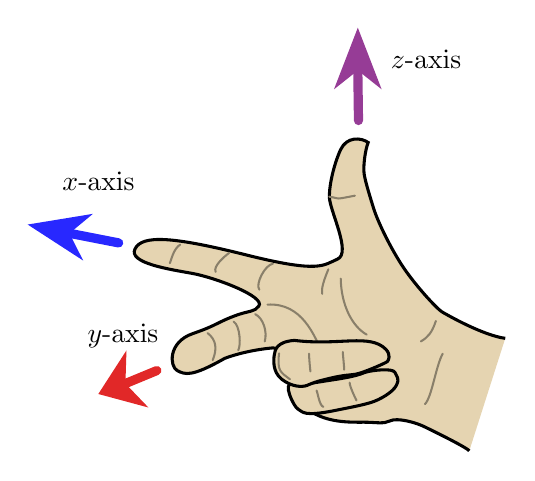
\begin{tikzpicture}[y=0.80pt, x=0.80pt, yscale=-1.000000, xscale=1.000000, inner sep=0pt, outer sep=0pt]
\path[draw=black,fill=ce5d4b1,line width=1.109pt] (197.7203,128.5199) ..
  controls (187.5579,127.1341) and (171.3905,117.8956) .. (169.0809,116.5099) ..
  controls (166.7713,115.1241) and (156.1470,103.5760) .. (150.6039,94.7994) ..
  controls (145.0608,86.0228) and (139.9796,75.3985) .. (138.1319,69.3935) ..
  controls (136.2842,63.3885) and (134.4365,57.3834) .. (133.9746,54.1500) ..
  controls (133.5127,50.9165) and (134.4365,43.2947) .. (135.8223,40.0612) ..
  controls (132.5888,37.7516) and (126.1219,37.2897) .. (123.3503,43.2947) ..
  controls (120.5788,49.2997) and (118.2691,58.5382) .. (118.2691,64.5433) ..
  controls (118.2691,70.5483) and (128.4315,89.9492) .. (121.9645,92.7207) ..
  controls (115.4976,95.4923) and (114.1118,99.1877) .. (80.8532,90.8730) ..
  controls (47.5946,82.5584) and (33.7368,81.6345) .. (30.5034,88.1015) ..
  controls (27.2699,94.5684) and (46.2088,97.3400) .. (56.3712,99.1877) ..
  controls (66.5335,101.0354) and (89.6395,109.6429) .. (86.3963,113.9693) ..
  controls (84.3869,116.6493) and (82.0658,116.0424) .. (76.8303,117.8901) ..
  controls (67.7715,121.0875) and (67.9114,122.4936) .. (56.6021,126.3641) ..
  controls (45.3159,130.2267) and (46.0504,141.2501) .. (49.5961,143.0996) ..
  controls (53.1419,144.9492) and (56.0705,146.0292) .. (71.0230,137.5505) ..
  controls (77.6516,135.0839) and (85.7039,133.4463) .. (92.7866,132.8306) ..
  controls (99.8693,132.2148) and (104.1813,158.6984) .. (111.8798,162.7019) ..
  controls (119.5782,166.7054) and (128.5086,166.3973) .. (134.0517,166.3973) ..
  controls (139.5948,166.3973) and (142.6740,167.3216) .. (145.7537,165.7816) ..
  controls (148.8333,164.2415) and (157.4561,166.3968) .. (162.0754,168.8607) ..
  controls (162.0754,168.8607) and (179.9366,177.4835) .. (181.4762,179.3312);
\path[draw=c897f6a,line cap=round,miter limit=4.00,line width=0.739pt]
  (90.3231,113.2759) .. controls (106.0281,112.3525) and (111.5712,127.4418) ..
  (115.2666,135.4488);
\path[draw=c897f6a,line cap=round,miter limit=4.00,line width=0.739pt]
  (123.4275,101.5735) .. controls (123.5817,113.2759) and (128.5091,123.1306) ..
  (135.1294,126.8251);
\path[draw=c897f6a,line cap=round,miter limit=4.00,line width=0.739pt]
  (92.7866,94.7989) .. controls (89.0912,95.4147) and (84.7800,104.0374) ..
  (86.6277,106.5009);
\path[draw=c897f6a,line cap=round,miter limit=4.00,line width=0.739pt]
  (73.0776,89.8716) .. controls (70.6142,91.7193) and (65.6868,96.0304) ..
  (66.9188,98.4943);
\path[draw=c897f6a,line cap=round,miter limit=4.00,line width=0.739pt]
  (50.9052,86.1762) .. controls (47.8256,88.0239) and (46.8246,93.3365) ..
  (46.2088,94.5679);
\path[draw=c897f6a,line cap=round,miter limit=4.00,line width=0.739pt]
  (84.7800,117.5875) .. controls (88.4754,119.4352) and (90.3231,125.5936) ..
  (89.0912,129.9052);
\path[draw=c897f6a,line cap=round,miter limit=4.00,line width=0.739pt]
  (74.9932,120.9466) .. controls (78.0729,122.7943) and (78.3413,132.0296) ..
  (77.1093,133.8773);
\path[draw=c897f6a,line cap=round,miter limit=4.00,line width=0.739pt]
  (63.2381,126.1188) .. controls (67.2329,129.1144) and (67.6685,133.2944) ..
  (65.5889,138.3441);
\path[draw=c897f6a,line cap=round,miter limit=4.00,line width=0.739pt]
  (117.8072,97.3400) .. controls (115.9595,101.9592) and (114.5737,105.6546) ..
  (115.0357,108.4262);
\path[draw=c897f6a,line cap=round,miter limit=4.00,line width=0.739pt]
  (118.2691,64.5433) .. controls (123.7878,65.3318) and (119.5057,66.0455) ..
  (129.8173,64.0813);
\path[draw=c897f6a,line cap=round,miter limit=4.00,line width=0.739pt]
  (166.3865,120.6672) .. controls (164.5388,126.2103) and (162.6911,128.0575) ..
  (159.6114,129.9052);
\path[draw=black,fill=ce5d4b1,line width=1.109pt] (120.5021,161.1628) ..
  controls (127.8490,159.6934) and (133.1283,158.6993) .. (137.1314,157.4674) ..
  controls (141.1344,156.2354) and (146.9852,152.8476) .. (148.5252,149.7685) ..
  controls (150.0653,146.6893) and (148.8333,146.0735) .. (147.9095,143.9177) ..
  controls (146.9856,141.7619) and (136.8238,142.9939) .. (134.3598,143.9177) ..
  controls (131.8959,144.8416) and (129.7406,145.7654) .. (119.5782,147.3050) ..
  controls (109.4159,148.8446) and (106.6443,149.6146) .. (101.4089,148.9984) ..
  controls (97.1167,148.4931) and (102.0255,159.3146) .. (104.1809,160.5466) ..
  controls (106.3362,161.7785) and (106.6443,163.9343) .. (120.5021,161.1628) --
  cycle;
\path[draw=black,fill=ce5d4b1,line width=1.109pt] (143.7845,133.4473) ..
  controls (146.1343,135.9107) and (145.1269,138.3746) .. (144.4557,138.9904) ..
  controls (143.7845,139.6061) and (136.0620,142.9934) .. (132.0331,144.2254) ..
  controls (128.0037,145.4573) and (127.3326,144.5335) .. (119.2752,146.3812) ..
  controls (111.2174,148.2289) and (110.5462,148.8446) .. (108.1955,149.7685) ..
  controls (105.8452,150.6923) and (101.1451,150.3842) .. (96.7808,146.9969) ..
  controls (92.4161,143.6096) and (93.0873,137.7584) .. (93.4231,135.9107) ..
  controls (93.7589,134.0630) and (94.0952,130.0595) .. (102.4884,129.4438) ..
  controls (122.7725,131.9811) and (136.5302,126.1649) .. (143.7845,133.4473) --
  cycle;
\path[draw=c897f6a,line cap=round,miter limit=4.00,line width=0.739pt]
  (95.5577,135.2950) .. controls (94.6694,143.2886) and (96.0699,143.6863) ..
  (100.4850,146.9969);
\path[draw=c897f6a,line cap=round,miter limit=4.00,line width=0.739pt]
  (109.1078,135.4483) .. controls (109.1078,137.9118) and (109.7235,143.4549) ..
  (109.7235,143.4549);
\path[draw=c897f6a,line cap=round,miter limit=4.00,line width=0.739pt]
  (124.3513,134.6783) .. controls (124.3513,135.9102) and (124.9675,140.8371) ..
  (124.9675,142.6848);
\path[draw=c897f6a,line cap=round,miter limit=4.00,line width=0.739pt]
  (127.4305,148.5370) .. controls (127.4305,150.3847) and (130.5102,156.5435) ..
  (130.5102,156.5435);
\path[draw=c897f6a,line cap=round,miter limit=4.00,line width=0.739pt]
  (112.4951,152.0781) .. controls (113.1108,153.3100) and (113.7270,158.8527) ..
  (115.5747,159.4689);
\path[draw=c897f6a,line cap=round,miter limit=4.00,line width=0.739pt]
  (169.4657,135.4488) .. controls (166.3865,140.9919) and (164.5388,155.1582) ..
  (161.4591,158.2374);
\path[draw=c963c96,line cap=round,line width=3.326pt] (131.4340,30.1298) --
  (131.1254,7.4955);
\path[cm={{0.46193,0.0,0.0,0.46193,(-17.99047,-11.80742)}},fill=c963c96]
  (322.8140,0.0000) -- (346.1270,60.3000) -- (322.8140,41.7880) --
  (299.5010,60.3000) -- cycle;
\path[draw=c2828ff,line cap=round,line width=3.326pt] (23.1190,85.4094) --
  (0.9023,81.0705);
\path[cm={{0.46193,0.0,0.0,0.46193,(-17.99047,-11.80742)}},fill=c2828ff]
  (0.0000,192.5000) -- (63.7990,182.0440) -- (40.9000,201.0670) --
  (54.2400,227.6800) -- cycle;
\path[draw=ce12828,line cap=round,line width=3.326pt] (40.3862,143.0553) --
  (26.1627,148.9449);
\path[cm={{0.46193,0.0,0.0,0.46193,(-17.99047,-11.80742)}},fill=ce12828]
  (69.0630,358.1970) -- (96.6050,315.5680) -- (95.5850,348.0050) --
  (118.0640,371.4130) -- cycle;
\begin{scope}[cm={{0.46193,0.0,0.0,0.46193,(-17.99047,-11.80742)}}]
\end{scope}
\path[fill=black,line join=miter,line cap=butt,line width=0.800pt]
  (-2.2839,61.9362) node[above right] (text4204) {$x$-axis};
\path[fill=black,line join=miter,line cap=butt,line width=0.800pt]
  (9.0458,132.6143) node[above right] (text4204-3) {$y$-axis};
\path[fill=black,line join=miter,line cap=butt,line width=0.800pt]
  (146.0527,6.4312) node[above right] (text4204-7) {$z$-axis};
\end{tikzpicture}\footnote{ Image credit: Acdx, from Wikipedia \url{https://en.wikipedia.org/wiki/Cross_product}}
\end{center}

We now have three standard basis vectors, $\xhat$, $\yhat$,
and $\zhat$, each pointing one unit in the positive direction of their
respective axes.
Any vector in three-dimensional
space can be represented 
in exactly one way
as a linear combination $\alpha\xhat+\beta\yhat+\gamma\zhat$.  Thus,
vectors in three-dimensional space, notated $\R^3$,
are synonymous with triplets $(\alpha,\beta,\gamma)$
of real numbers.  With some clever geometry, we deduce
\[
	\norm{\alpha\xhat+\beta\yhat+\gamma\zhat}=\sqrt{\alpha^2+\beta^2+\gamma^2}.
\]

Historically, three-dimensional space has been studied a lot and there
are several notations for the standard basis vectors still in use.

The following is a non-exhaustive list.
\begin{center}
	\begin{tabular}{c  c  c}
		$\hat{\mathbf{x}}$ & $\hat{\mathbf{y}}$ &$\hat{\mathbf{z}}$\\
		$\hat{\imath}$ & $\hat{\jmath}$ &$\hat{k}$\\
		$\mathbf{i}$ & $\mathbf j$ & $\mathbf k$\\
		$\vec e_1$ & $\vec e_2$ & $\vec e_3$
	\end{tabular}
\end{center}
Keep these notations in the back of your mind.  You might see them in other classes.

\subsection{Higher dimensions}
One can't progress very far in the study of science and mathematics
without encountering a need for higher dimensional ``vectors''.  For
example, physicists have known since Einstein that the physical
universe is best thought of as a four-dimensional entity called
spacetime in which time plays a role close to that of the 
three spatial coordinates.  Since we don't have any way to deal with
$\R^n$\index{$\R^n$}
intuitively, we must
proceed by analogy with two and three dimensions.
The easiest
way to proceed is to generalize the idea of a standard basis.
From there, we can represent vectors in $\R^n$ as $n$-tuples of real numbers.
We then define
\[
	\norm{(x_1,x_2,\ldots,x_n)} = \sqrt{x_1^2+x_2^2+\cdots+x_n^2}.	
\]
We've now unified our theory of vectors across all integer dimensions $n>0$.
The case $n=1$ yields  ``geometry'' on a line, 
the cases $n = 2$ and $n = 3$ geometry in the plane and in space, and
the case $n = 4$ yields the geometry of ``4-vectors'' which
are  used in the special theory of relativity.
Larger values of $n$ are used in a
variety of contexts, some of which we shall encounter later.


\begin{exercises}
	\begin{enumerate}
		\item Find $\norm{a}$, $5\vec a-2\vec b$, and $-3\vec b$ for each of
			the following vector pairs.
			\begin{enumerate}
				\item $\vec a=2\xhat+3\yhat$, $\vec b=4\xhat-9\yhat$
				\item $\vec a=(1,2,-1)$, $\vec b=(2,-1,0)$
			\end{enumerate}
		\item Let $P=(7,2,9)$ and $Q=(-2,1,4)$.  Find $\overrightarrow{PQ}$
			as a linear combination of $\xhat$, $\yhat$, and $\zhat$.
	\end{enumerate}
\end{exercises}


\section{Dot Products \& Projections}
\subsection{Dot Product}
Let $\vec a$ and $\vec b$ be vectors.  We assume they are placed so their
tails coincide.  Let $\theta$ denote the \emph{smaller} of the
two angles between them, so $0\le \theta \le \pi$.
The \emph{dot product}\index{dot product} of $\vec a$ and $\vec b$ is defined to be
\[
	\vec a\cdot \vec b=\norm{\vec a}\norm{\vec b}\cos \theta.
\]
We will call this the \emph{geometric definition of the dot product}.
The dot product is also sometimes called the \emph{scalar product} because
the result is a scalar.
Note that $\vec a\cdot\vec b = 0$ when either $\vec a$ or $\vec b$ is zero or,
more interestingly, if their directions are perpendicular.

\begin{center}
	\newcommand{\tikzAngleOfLine}{\tikz@AngleOfLine}                               
	  \def\tikz@AngleOfLine(#1)(#2)#3{%                                            
	  \pgfmathanglebetweenpoints{%                                                 
	    \pgfpointanchor{#1}{center}}{%                                             
	    \pgfpointanchor{#2}{center}}                                               
	  \pgfmathsetmacro{#3}{\pgfmathresult}%                                        
	  }                                                                            
	\newcommand{\tikzMarkAngle}[3]{                                                
	\tikzAngleOfLine#1#2{\AngleStart}                                              
	\tikzAngleOfLine#1#3{\AngleEnd}                                                
	\draw #1+(\AngleStart:0.35cm) arc (\AngleStart:\AngleEnd:0.35cm);              
	} 
	\usetikzlibrary{patterns,decorations.pathreplacing}
	\begin{tikzpicture}
		\coordinate (A) at (2,1);
		\coordinate (B) at (.5,2);
		\coordinate (O) at (0,0);

		%\draw [mypink,fill] (A) circle (1.5pt) node [right] {initial point};
		%\draw [mypink,fill] (B) circle (1.5pt) node [left] {terminal point};
		\draw[->,thick,myred!60!white] (0,0) -- +(A) node [midway,below right] {$\vec a$};
		\draw[->,thick,mypink] (0,0) -- +(B) node [midway,above left] {$\vec b$};
		\tikzMarkAngle{(O)}{(A)}{(B)}
		\node at ($(O)+(50:.65)$) {$\theta$};
	\end{tikzpicture}
	\hspace{1cm}
	\begin{tikzpicture}
		\coordinate (A) at (-2,-1);
		\coordinate (B) at (.5,2);
		\coordinate (O) at (0,0);

		%\draw [mypink,fill] (A) circle (1.5pt) node [right] {initial point};
		%\draw [mypink,fill] (B) circle (1.5pt) node [left] {terminal point};
		\draw[->,thick,myred!60!white] (0,0) -- +(A) node [midway,below right] {$\vec a$};
		\draw[->,thick,mypink] (0,0) -- +(B) node [midway,above left] {$\vec b$};
		\tikzMarkAngle{(O)}{(B)}{(A)}
		\node at ($(O)+(140:.65)$) {$\theta$};
	\end{tikzpicture}
\end{center}

Algebraically, we can define the dot product in terms of components:
\[
	\mat{a_1\\a_2\\\vdots\,\,\,\, \\a_n}\cdot \mat{b_1\\b_2\\\vdots\,\,\,\,\\b_n}
	=a_1b_1+a_2b_2+\cdots+a_nb_n.
\]
We will call this the \emph{algebraic definition of the dot product}\footnote{
	Philosophically,
every object should have only one definition from which equivalent characterizations
can be deduced as theorems.  If you're bothered, pick your favorite definition
to be the ``true'' definition and consider the other definition a theorem.
}.

By switching between algebraic and geometric definitions, we can use the dot
product to find quantities that are otherwise difficult.
\begin{example}
	Find the angle between the vectors $\vec v=(1,2,3)$ and $\vec w=(1,1,-2)$.

	From the algebraic definition of the dot product, we know
	\[
		\vec v\cdot \vec w = 1(1)+2(1)+3(-2) = -3.
	\]
	From the geometric definition, we know
	\[
		\vec v\cdot \vec w=\norm{\vec v}\norm{\vec w}\cos\theta
		=\sqrt{14}\sqrt{6}\cos\theta=\sqrt{21}\cos\theta.
	\]
	Equating the two definitions of $\vec v\cdot \vec w$, we see
	\[
		\cos\theta = \frac{-3}{\sqrt{21}}
	\]
	and so $\theta=\arccos(-3/\sqrt{21})$.
\end{example}

Recall that for vectors $\vec a$, $\vec b$ the relationship $\vec a\cdot \vec b=0$
can hold for two reasons: (i) either $\vec a=\vec 0$, $\vec b=\vec 0$, or both
or (ii) $\vec a$ and $\vec b$ meet at $90^{\circ}$.  Thus, the dot product
can be used to tell if two vectors are perpendicular.  There is some strangeness
with the zero vector here, but it turns out this strangeness simplifies our lives
mathematically.

\begin{definition}[Orthogonal]
	The vectors $\vec u$ and $\vec v$ are \emph{orthogonal}\index{orthogonal}
	if $\vec u\cdot\vec v=0$.
\end{definition}

The definition of orthogonal encapsulates both the idea of two vectors being
perpendicular and the idea of one of them being $\vec 0$.

Before we continue, let's pin down the idea of one vector pointing
in the \emph{direction} of another.  There are many ways we could define
this idea, but we'll go with this one.

\begin{definition}
	The vector $\vec u$ points in the \emph{direction} of
	the vector $\vec v$ if $k\vec u=\vec v$ for some scalar $k$.
\end{definition}

A simple example is that $2\xhat$ points in the direction of $\xhat$ since 
$\frac{1}{2}(2\xhat)=\xhat$.  However, nothing in the definition says the
scalar needs to be positive, so $-\xhat$ also points in the direction $\xhat$.

\subsection{Projection}
Another common vector operation is \emph{projection}\index{projection}.
Projection measures how much a vector points in the direction
of another.  This quantity is encoded as a vector.  We make this
definition mathematically precise as follows.

\begin{definition}[Projection]
	For a vector $\vec u$ and a non-zero vector $\vec v$,
	the \emph{projection} of $\vec u$ onto $\vec v$ is written
	as $\Proj_{\vec v}\vec u$ and is a vector in the direction
	of $\vec v$ with the property that $\vec u-\Proj_{\vec v}\vec u$
	is orthogonal to $\vec v$.

	The vector $\vec u-\Proj_{\vec v}\vec u$ is called the
	\emph{perpendicular component} of the projection of $\vec u$
	onto $\vec v$ and is notated $\Perp_{\vec v}\vec u$.
\end{definition}

We can visualize
projections with the following diagram.

	\begin{center}
	\usetikzlibrary{patterns,decorations.pathreplacing}
	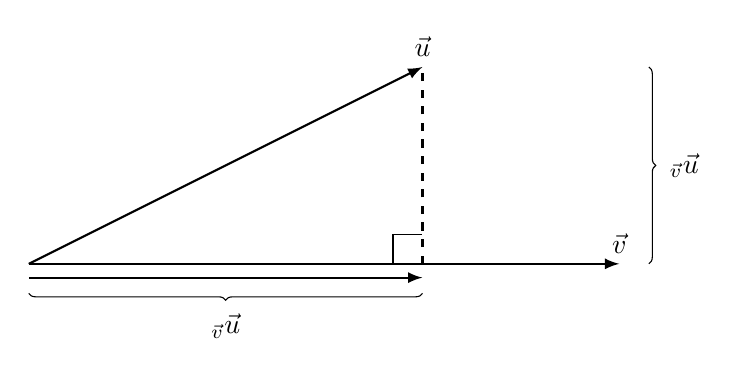
\begin{tikzpicture}[>=latex,scale=2.5]
		\draw[->,thick,black] (0,0) -- (2,1) node [above] {$\vec u$};
		\draw[->,thick,black] (0,0) -- (3,0) node [above] {$\vec v$};
		\draw[->,thick,black,yshift=-.07cm] (0,0) -- (2,0);
		\draw[decoration={brace, mirror}, decorate, yshift=-.15cm] (0,0) -- (2,0) node [midway,below,yshift=-4pt] {$\Proj_{\vec v}\vec u$};
		
		\draw[dashed,thick,black] (2,0) -- (2,1);
		\draw[decoration={brace, mirror}, decorate, xshift=1.15cm] (2,0) -- (2,1) node [midway,right,xshift=4pt] {$\Perp_{\vec v}\vec u$};
		\draw[thin,black] (1.85,0)--(1.85,.15)--(2,.15);

	\end{tikzpicture}
	\end{center}

From the picture it appears that $\vec u$, $\Proj_{\vec v}\vec u$,
and $\Perp_{\vec v}\vec u$ form a right triangle.  Of course, we shouldn't
trust the picture. We should verify this mathematically.

\begin{theorem}
	If $\vec u$ and $\vec v$ are non-zero vectors, then $\vec v$, $\Proj_{\vec v}\vec u$,
	and $\Perp_{\vec v}\vec u$ form a (possibly degenerate) right triangle.
\end{theorem}
\begin{proof}
	We need to verify that the sides $\Proj_{\vec v}\vec u$ and $\Perp_{\vec v}\vec u$
	meet at a right angle and that the hypotenuse $\vec u$ meets the sides.  That is,
	$\Perp_{\vec v}\vec u+\Proj_{\vec v}\vec u=\vec u$.

	By the definition of projection, $\Perp_{\vec v}\vec u=\vec u-\Proj_{\vec v}\vec u$
	is orthogonal to $\vec v$.  Since $\Proj_{\vec v}\vec u$ points in the
	direction of $\vec v$, we have $\Proj_{\vec v}\vec u=k\vec v$ and so
	$\Perp_{\vec v}\vec u$ is orthogonal to $\Proj_{\vec v}\vec u$.

	Finally, consider
	\[
		\Perp_{\vec v}\vec u+\Proj_{\vec v}\vec u=
		(\vec u-\Proj_{\vec v}\vec u)+\Proj_{\vec v}\vec u=\vec u,
	\]
	so indeed the vectors form a right triangle.
\end{proof}

Now that we've proved $\vec u$, $\Proj_{\vec v}\vec u$,
and $\Perp_{\vec v}\vec u$ form a right triangle, we are free to use
trigonometry to compute projections.  If $\theta$ is the angle between $\vec u$
and $\vec v$ and $0\leq \theta\leq \pi/2$, 
we know $\norm{\Proj_{\vec v}\vec u}=\norm{\vec u}\cos\theta$.  This means
\[
	\Proj_{\vec v}\vec u = k\vec v=\norm{\vec u}\cos\theta\frac{\vec v}{\norm{\vec v}}
\]
(Recall that $\vec v/\norm{\vec v}$ is a unit vector in the direction of $\vec v$).
But $\cos \theta$ appears in the formula for the dot product.  Solving for
$\cos\theta$ in the dot product formula, we see $\cos\theta=\frac{\vec u\cdot\vec v}{\norm{\vec u}\norm{\vec v}}$.
Thus,
\[
	\Proj_{\vec v}\vec u = \norm{\vec u}\cos\theta\vec v
	=\frac{\vec u\cdot \vec v}{\norm{\vec u}\norm{\vec v}}\left(\frac{\vec v}{\norm{\vec v}}\right)
	=\frac{\vec u\cdot \vec v}{\norm{\vec v}^2}\vec v.
\]
Upon close inspection, we see $\norm{\vec v}^2=\vec v\cdot \vec v$ (since $\cos 0=1$)
and so we finally arrive at the formula
\[
	\Proj_{\vec v}\vec u  
	=\frac{\vec u\cdot \vec v}{\vec v\cdot \vec v}\vec v
\]
Incredibly, if we use the algebraic definition of the dot product, we can
compute a projection without computing cosine of anything!

\begin{exercises}
\end{exercises}

\section{The Cross Product}

For vectors $\vec a$ and $\vec b$, the dot $\vec a\cdot \vec b$ measures
how close $\vec a$ and $\vec b$ are to being orthogonal.  In contrast,
the \emph{cross product}\index{cross product} of $\vec a$ and $\vec b$,
written $\vec a\times \vec b$ will
measure the \emph{area} of the parallelogram whose sides are given by $\vec a$ and
$\vec b$.

Let's explore this idea.  Since the cross product is a \emph{product}, we will
demand it follow reasonable distribution laws\footnote{ The technical term
for satisfying these laws is \emph{bilinearity}.}:
\begin{align*}
	\vec a\times (\vec b+\vec c) &= \vec a\times \vec b+\vec a\times\vec c\\
	(\vec a+\vec b)\times\vec c &= \vec a\times \vec c+\vec b\times \vec c\\
	(\alpha\vec a)\times \vec b &= \alpha(\vec a\times \vec b)\\
	\vec a\times(\alpha \vec b) &= \alpha(\vec a\times \vec b)
\end{align*}
for vectors $\vec a$, $\vec b$, $\vec c$ and scalars $\alpha$.

Now, suppose $\vec a\times \vec b$ indeed encapsulates the area of the parallelogram
with sides $\vec a$ and $\vec b$.  If we slide the tip of $\vec b$ parallel to the vector
$\vec a$, we should not change the area.  Thus the cross product of $\vec a$ and $\vec b$
should be the same as that of $\vec a$ and $\vec b+\alpha\vec a$.  

\begin{center}
	\usetikzlibrary{patterns,decorations.pathreplacing}
	\begin{tikzpicture}
		\coordinate (A) at (2,0);
		\coordinate (B) at (1,2);
		\coordinate (O) at (0,0);

		%\draw [mypink,fill] (A) circle (1.5pt) node [right] {initial point};
		%\draw [mypink,fill] (B) circle (1.5pt) node [left] {terminal point};
		\draw[fill,gray!30!white] (O) -- +(B) -- +($(A)+(B)$) -- +(A) -- (O);
		\draw[->,thick,myred!60!white] (0,0) -- +(A) node [midway,below] {$\vec a$};
		\draw[->,thick,mypink] (0,0) -- +(B) node [midway,above left] {$\vec b$};
		\draw[black,dashed,<->] ($.6*(A)$) -- ($.6*(A)+(0,2)$) node [midway,right] {height};
	\end{tikzpicture}
	\hspace{1cm}
	\begin{tikzpicture}
		\coordinate (A) at (2,0);
		\coordinate (B) at (1,2);
		\coordinate (C) at ($(B)+2*(A)$);
		\coordinate (O) at (0,0);

		%\draw [mypink,fill] (A) circle (1.5pt) node [right] {initial point};
		%\draw [mypink,fill] (B) circle (1.5pt) node [left] {terminal point};
		\draw[fill,gray!30!white] (O) -- +(C) -- +($(A)+(C)$) -- +(A) -- (O);
		\draw[->,thick,myred!60!white] (0,0) -- +(A) node [midway,below] {$\vec a$};
		\draw[->,thick,gray,dashed] (0,0) -- +(B);% node [midway,above left] {$\vec b$};
		\draw[->,thick,gray,dashed] (B) -- +($2*(A)$);% node [midway,above] {$2\vec a$};
		\draw[->,thick,mypink] (0,0) -- +(C) node [midway,above left] {$\vec b+2\vec a$};
		\draw[black,dashed,<->] ($2.6*(A)$) -- ($2.6*(A)+(0,2)$) node [midway,right] {height};
	\end{tikzpicture}
\end{center}

Using this invariance along with our distributive rules,
we now see
\[
	\vec a\times \vec b = \vec a\times (\vec b+\alpha\vec a)=
	\vec a\times \vec b+\alpha(\vec a\times\vec a),
\]
and so $\vec a\times \vec a=0$.  We can apply this newly-found fact to
the vector $\vec a+\vec b$ to deduce
\begin{align*}
	0=(\vec a+\vec b)\times (\vec a+\vec b)&=
	\vec a\times \vec a+\vec a\times\vec b+\vec b\times \vec a+\vec b\times \vec b\\
	&=0+\vec a\times \vec b+\vec b\times \vec a+0\\
	&=\vec a\times \vec b+\vec b\times \vec a,
\end{align*}
and so 
\[
	\vec a\times \vec b=-\vec b\times \vec a.
\]
Products with this property are called \emph{anti-commutative}.  Now
for an incredible fact of the universe: the result of the cross product of
two vectors in $\R^3$ can be represented by another vector in $\R^3$ whose magnitude
corresponds to the area of the parallelogram
with sides $\vec a$ and $\vec b$.\footnote{ This is \emph{only} true in $\R^3$.  In $\R^4$ a product that
produces area-like quantities does exist, but the output cannot be described by
a vector.  In higher dimensions, the cross product is called the \emph{wedge product}.}
Using trigonometry, we deduce
\[
	\norm{\vec a\times \vec b}=\norm{\vec a}\norm{\vec b}\sin \theta
\]
where $0\leq \theta\leq \pi$ is smaller of the two angles between $\vec a$ and $\vec b$.
What remains to be seen is what direction $\vec a\times \vec b$ points in.  For this,
we use the standard basis for $\R^3$ as a launching point. Recall
$\xhat$, $\yhat$, and $\zhat$ are all unit vectors and all orthogonal to each other.
Thus, any of them cross each other must result in a unit vector.  By convention,
\begin{align*}
	\xhat\times\yhat &=  \zhat, \\
	\yhat\times\zhat &=  \xhat\\
	\zhat\times\xhat &=  \yhat.
\end{align*}
Let $\vec a=a_x\xhat +a_y\yhat +a_z\zhat$ and $\vec b=b_x\xhat +b_y\yhat +b_z\zhat$.
Using the distributive laws of the cross product we see,
\begin{align*}
	\vec a\times\vec b &= (a_x \xhat + a_y\yhat + a_z\zhat) \times (b_x\xhat + b_y\yhat + b_z\zhat) \\
	&= \phantom{+}a_xb_x\xhat\times\xhat + a_xb_y\xhat\times\yhat + a_xb_z\xhat\times\zhat \\
       &\phantom{=}+ a_yb_x\yhat\times\xhat + a_yb_y\yhat\times\yhat + a_yb_z\yhat\times\zhat \\
       &\phantom{=}+ a_zb_x\zhat\times\xhat + a_zb_y\zhat\times\yhat + a_zb_z\zhat\times\zhat \\
	&= \phantom{+}\vec 0  + a_xb_y\zhat - a_xb_z\yhat \\
       &\phantom{=}- a_yb_x\zhat + \vec 0 + a_yb_z \xhat \\
	&\phantom{=}+ a_zb_x\yhat - a_zb_y\xhat + {\vec 0}\\
\intertext{so}
\vec a\times \vec b &= (a_yb_z - a_zb_y)\xhat - (a_xb_z - a_zb_x)\yhat + (a_xb_y - a_yb_x)\zhat.
\end{align*}

\begin{exercise}
	Verify that $\norm{\vec a\times \vec b}=\norm{\vec a}\norm{\vec b}\sin\theta$. (Hint: you
	can use $\vec a\cdot \vec b=\norm{\vec a}\norm{\vec b}\cos\theta$ to solve for $\theta$
	and the proceed using components.)
\end{exercise}

Now that we know what the cross product is and how to compute it, let's explore
some of its incredible properties.  First,
\[
	(\vec a\times\vec b)\cdot \vec a=(a_yb_z - a_zb_y)a_x - (a_xb_z - a_zb_x)a_y + (a_xb_y - a_yb_x)a_z=0
\]
and 
\[
	(\vec a\times\vec b)\cdot \vec b=(a_yb_z - a_zb_y)b_x - (a_xb_z - a_zb_x)b_y + (a_xb_y - a_yb_x)b_z=0.
\]
Thus, $\vec a\times\vec b$ is orthogonal to both $\vec a$ and $\vec b$.  
Just based on this property, since the length of $\vec a\times \vec b$ is fixed, $\vec a\times\vec b$
can be one of two vectors in space.
If we investigate further, we'll
see that $\vec a\times\vec b$ is the vector that satisfies the \emph{right-hand rule}.

\begin{center}
\definecolor{ce5d4b1}{RGB}{229,212,177}
\definecolor{c897f6a}{RGB}{137,127,106}
\definecolor{c963c96}{RGB}{150,60,150}
\definecolor{c2828ff}{RGB}{40,40,255}
\definecolor{ce12828}{RGB}{225,40,40}

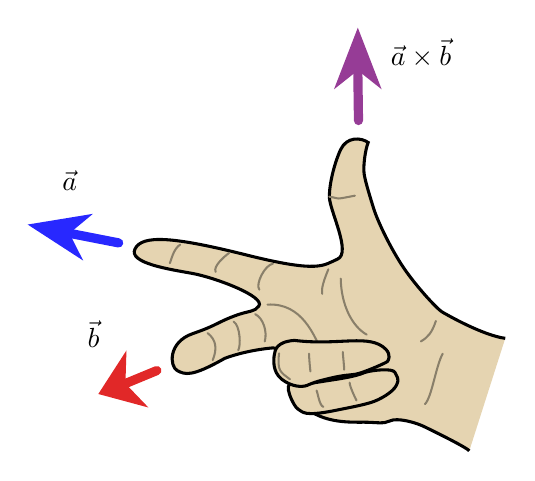
\begin{tikzpicture}[y=0.80pt, x=0.80pt, yscale=-1.000000, xscale=1.000000, inner sep=0pt, outer sep=0pt]
\path[draw=black,fill=ce5d4b1,line width=1.109pt] (197.7203,128.5199) ..
  controls (187.5579,127.1341) and (171.3905,117.8956) .. (169.0809,116.5099) ..
  controls (166.7713,115.1241) and (156.1470,103.5760) .. (150.6039,94.7994) ..
  controls (145.0608,86.0228) and (139.9796,75.3985) .. (138.1319,69.3935) ..
  controls (136.2842,63.3885) and (134.4365,57.3834) .. (133.9746,54.1500) ..
  controls (133.5127,50.9165) and (134.4365,43.2947) .. (135.8223,40.0612) ..
  controls (132.5888,37.7516) and (126.1219,37.2897) .. (123.3503,43.2947) ..
  controls (120.5788,49.2997) and (118.2691,58.5382) .. (118.2691,64.5433) ..
  controls (118.2691,70.5483) and (128.4315,89.9492) .. (121.9645,92.7207) ..
  controls (115.4976,95.4923) and (114.1118,99.1877) .. (80.8532,90.8730) ..
  controls (47.5946,82.5584) and (33.7368,81.6345) .. (30.5034,88.1015) ..
  controls (27.2699,94.5684) and (46.2088,97.3400) .. (56.3712,99.1877) ..
  controls (66.5335,101.0354) and (89.6395,109.6429) .. (86.3963,113.9693) ..
  controls (84.3869,116.6493) and (82.0658,116.0424) .. (76.8303,117.8901) ..
  controls (67.7715,121.0875) and (67.9114,122.4936) .. (56.6021,126.3641) ..
  controls (45.3159,130.2267) and (46.0504,141.2501) .. (49.5961,143.0996) ..
  controls (53.1419,144.9492) and (56.0705,146.0292) .. (71.0230,137.5505) ..
  controls (77.6516,135.0839) and (85.7039,133.4463) .. (92.7866,132.8306) ..
  controls (99.8693,132.2148) and (104.1813,158.6984) .. (111.8798,162.7019) ..
  controls (119.5782,166.7054) and (128.5086,166.3973) .. (134.0517,166.3973) ..
  controls (139.5948,166.3973) and (142.6740,167.3216) .. (145.7537,165.7816) ..
  controls (148.8333,164.2415) and (157.4561,166.3968) .. (162.0754,168.8607) ..
  controls (162.0754,168.8607) and (179.9366,177.4835) .. (181.4762,179.3312);
\path[draw=c897f6a,line cap=round,miter limit=4.00,line width=0.739pt]
  (90.3231,113.2759) .. controls (106.0281,112.3525) and (111.5712,127.4418) ..
  (115.2666,135.4488);
\path[draw=c897f6a,line cap=round,miter limit=4.00,line width=0.739pt]
  (123.4275,101.5735) .. controls (123.5817,113.2759) and (128.5091,123.1306) ..
  (135.1294,126.8251);
\path[draw=c897f6a,line cap=round,miter limit=4.00,line width=0.739pt]
  (92.7866,94.7989) .. controls (89.0912,95.4147) and (84.7800,104.0374) ..
  (86.6277,106.5009);
\path[draw=c897f6a,line cap=round,miter limit=4.00,line width=0.739pt]
  (73.0776,89.8716) .. controls (70.6142,91.7193) and (65.6868,96.0304) ..
  (66.9188,98.4943);
\path[draw=c897f6a,line cap=round,miter limit=4.00,line width=0.739pt]
  (50.9052,86.1762) .. controls (47.8256,88.0239) and (46.8246,93.3365) ..
  (46.2088,94.5679);
\path[draw=c897f6a,line cap=round,miter limit=4.00,line width=0.739pt]
  (84.7800,117.5875) .. controls (88.4754,119.4352) and (90.3231,125.5936) ..
  (89.0912,129.9052);
\path[draw=c897f6a,line cap=round,miter limit=4.00,line width=0.739pt]
  (74.9932,120.9466) .. controls (78.0729,122.7943) and (78.3413,132.0296) ..
  (77.1093,133.8773);
\path[draw=c897f6a,line cap=round,miter limit=4.00,line width=0.739pt]
  (63.2381,126.1188) .. controls (67.2329,129.1144) and (67.6685,133.2944) ..
  (65.5889,138.3441);
\path[draw=c897f6a,line cap=round,miter limit=4.00,line width=0.739pt]
  (117.8072,97.3400) .. controls (115.9595,101.9592) and (114.5737,105.6546) ..
  (115.0357,108.4262);
\path[draw=c897f6a,line cap=round,miter limit=4.00,line width=0.739pt]
  (118.2691,64.5433) .. controls (123.7878,65.3318) and (119.5057,66.0455) ..
  (129.8173,64.0813);
\path[draw=c897f6a,line cap=round,miter limit=4.00,line width=0.739pt]
  (166.3865,120.6672) .. controls (164.5388,126.2103) and (162.6911,128.0575) ..
  (159.6114,129.9052);
\path[draw=black,fill=ce5d4b1,line width=1.109pt] (120.5021,161.1628) ..
  controls (127.8490,159.6934) and (133.1283,158.6993) .. (137.1314,157.4674) ..
  controls (141.1344,156.2354) and (146.9852,152.8476) .. (148.5252,149.7685) ..
  controls (150.0653,146.6893) and (148.8333,146.0735) .. (147.9095,143.9177) ..
  controls (146.9856,141.7619) and (136.8238,142.9939) .. (134.3598,143.9177) ..
  controls (131.8959,144.8416) and (129.7406,145.7654) .. (119.5782,147.3050) ..
  controls (109.4159,148.8446) and (106.6443,149.6146) .. (101.4089,148.9984) ..
  controls (97.1167,148.4931) and (102.0255,159.3146) .. (104.1809,160.5466) ..
  controls (106.3362,161.7785) and (106.6443,163.9343) .. (120.5021,161.1628) --
  cycle;
\path[draw=black,fill=ce5d4b1,line width=1.109pt] (143.7845,133.4473) ..
  controls (146.1343,135.9107) and (145.1269,138.3746) .. (144.4557,138.9904) ..
  controls (143.7845,139.6061) and (136.0620,142.9934) .. (132.0331,144.2254) ..
  controls (128.0037,145.4573) and (127.3326,144.5335) .. (119.2752,146.3812) ..
  controls (111.2174,148.2289) and (110.5462,148.8446) .. (108.1955,149.7685) ..
  controls (105.8452,150.6923) and (101.1451,150.3842) .. (96.7808,146.9969) ..
  controls (92.4161,143.6096) and (93.0873,137.7584) .. (93.4231,135.9107) ..
  controls (93.7589,134.0630) and (94.0952,130.0595) .. (102.4884,129.4438) ..
  controls (122.7725,131.9811) and (136.5302,126.1649) .. (143.7845,133.4473) --
  cycle;
\path[draw=c897f6a,line cap=round,miter limit=4.00,line width=0.739pt]
  (95.5577,135.2950) .. controls (94.6694,143.2886) and (96.0699,143.6863) ..
  (100.4850,146.9969);
\path[draw=c897f6a,line cap=round,miter limit=4.00,line width=0.739pt]
  (109.1078,135.4483) .. controls (109.1078,137.9118) and (109.7235,143.4549) ..
  (109.7235,143.4549);
\path[draw=c897f6a,line cap=round,miter limit=4.00,line width=0.739pt]
  (124.3513,134.6783) .. controls (124.3513,135.9102) and (124.9675,140.8371) ..
  (124.9675,142.6848);
\path[draw=c897f6a,line cap=round,miter limit=4.00,line width=0.739pt]
  (127.4305,148.5370) .. controls (127.4305,150.3847) and (130.5102,156.5435) ..
  (130.5102,156.5435);
\path[draw=c897f6a,line cap=round,miter limit=4.00,line width=0.739pt]
  (112.4951,152.0781) .. controls (113.1108,153.3100) and (113.7270,158.8527) ..
  (115.5747,159.4689);
\path[draw=c897f6a,line cap=round,miter limit=4.00,line width=0.739pt]
  (169.4657,135.4488) .. controls (166.3865,140.9919) and (164.5388,155.1582) ..
  (161.4591,158.2374);
\path[draw=c963c96,line cap=round,line width=3.326pt] (131.4340,30.1298) --
  (131.1254,7.4955);
\path[cm={{0.46193,0.0,0.0,0.46193,(-17.99047,-11.80742)}},fill=c963c96]
  (322.8140,0.0000) -- (346.1270,60.3000) -- (322.8140,41.7880) --
  (299.5010,60.3000) -- cycle;
\path[draw=c2828ff,line cap=round,line width=3.326pt] (23.1190,85.4094) --
  (0.9023,81.0705);
\path[cm={{0.46193,0.0,0.0,0.46193,(-17.99047,-11.80742)}},fill=c2828ff]
  (0.0000,192.5000) -- (63.7990,182.0440) -- (40.9000,201.0670) --
  (54.2400,227.6800) -- cycle;
\path[draw=ce12828,line cap=round,line width=3.326pt] (40.3862,143.0553) --
  (26.1627,148.9449);
\path[cm={{0.46193,0.0,0.0,0.46193,(-17.99047,-11.80742)}},fill=ce12828]
  (69.0630,358.1970) -- (96.6050,315.5680) -- (95.5850,348.0050) --
  (118.0640,371.4130) -- cycle;
\begin{scope}[cm={{0.46193,0.0,0.0,0.46193,(-17.99047,-11.80742)}}]
\end{scope}
\path[fill=black,line join=miter,line cap=butt,line width=0.800pt]
  (-2.2839,61.9362) node[above right] (text4204) {$\vec a$};
\path[fill=black,line join=miter,line cap=butt,line width=0.800pt]
  (9.0458,132.6143) node[above right] (text4204-3) {$\vec b$};
\path[fill=black,line join=miter,line cap=butt,line width=0.800pt]
  (146.0527,6.4312) node[above right] (text4204-7) {$\vec a\times \vec b$};
\end{tikzpicture}\footnote{ Image credit: Acdx, from Wikipedia \url{https://en.wikipedia.org/wiki/Cross_product}}
\end{center}

A vector that encodes area, points orthogonally to others, and obeys the right-hand
rule is handy indeed, and the cross product will be a useful tool for solving
many problems.


\begin{exercises}
\end{exercises}


\section{Lines and Planes}

With a handle on vectors, we can now use them to describe some common geometric
objects: lines and planes.

\subsection{Lines}
Consider for a moment the line $\ell$ through the points $P$ and $Q$.  If $P,Q\in\R^2$, we
could describe this line in $y=mx+b$ form (provided it isn't a vertical line), but if
$P,Q\in\R^3$ it's much harder to describe $\ell$ with an equation.  Using vectors
provides an easier way.

Let $\vec d=\overrightarrow{PQ}$ and consider the set of points (or vectors)
\[
	\vec x=t\vec d+P
\]
for $t\in \R$.  Geometrically, this is the set of all points we get by starting at $P$ and
displacing by some multiple of the direction $\vec d$.  This is a line!


\begin{center}
	\usetikzlibrary{patterns,decorations.pathreplacing}
	\begin{tikzpicture}
		\coordinate (A) at (1,1);
		\coordinate (B) at (3,2);
		\coordinate (D) at ($(B)-(A)$);
		\begin{axis}[
		    anchor=origin,
		    disabledatascaling,
		    xmin=-1,xmax=5,
		    ymin=-1,ymax=3,
		    x=1cm,y=1cm,
		    grid=both,
		    grid style={line width=.1pt, draw=gray!10},
		    %major grid style={line width=.2pt,draw=gray!50},
		    axis lines=middle,
		    minor tick num=0,
		    enlargelimits={abs=0.5},
		    axis line style={latex-latex},
		    ticklabel style={font=\tiny,fill=white},
		    xlabel style={at={(ticklabel* cs:1)},anchor=north west},
		    ylabel style={at={(ticklabel* cs:1)},anchor=south west}
		]

		\draw [mypink,fill] (A) circle (1.5pt) node [below right] {$P$};
		\draw [mypink,fill] (B) circle (1.5pt) node [below right] {$Q$};
		\draw[->,thick,myred!60!white] (A) -- (B) node [midway,below right,yshift=2pt] {$\vec d$};


		\end{axis}
		\foreach \x in {-1,5} {
			\draw [mypink,fill] ($(A)+\x/3*(D)$) circle (1.5pt) node [left] {\footnotesize$\tfrac{\x}{3}\vec d+P$};
		}
		\foreach \x in {-3,-2,4,6} {
			\draw [mypink,fill] ($(A)+\x/3*(D)$) circle (1.5pt);
		}
	\end{tikzpicture}
	\begin{tikzpicture}
		\coordinate (A) at (1,1);
		\coordinate (B) at (3,2);
		\coordinate (D) at ($(B)-(A)$);
		\begin{axis}[
		    anchor=origin,
		    disabledatascaling,
		    xmin=-1,xmax=5,
		    ymin=-1,ymax=3,
		    x=1cm,y=1cm,
		    grid=both,
		    grid style={line width=.1pt, draw=gray!10},
		    %major grid style={line width=.2pt,draw=gray!50},
		    axis lines=middle,
		    minor tick num=0,
		    enlargelimits={abs=0.5},
		    axis line style={latex-latex},
		    ticklabel style={font=\tiny,fill=white},
		    xlabel style={at={(ticklabel* cs:1)},anchor=north west},
		    ylabel style={at={(ticklabel* cs:1)},anchor=south west}
		]

		\draw [mypink,fill] (A) circle (1.5pt) node [below right] {$P$};
		\draw [mypink,fill] (B) circle (1.5pt) node [below right] {$Q$};
		\draw[->,thick,myred!60!white] (A) -- (B) node [midway,below right,yshift=2pt] {$\vec d$};

		\end{axis}

		\foreach \x in {-3,-2,-1,0,4,5,6} {
			\draw [->, gray!50!white] (0,0) -- ($(A)+\x/3*(D)$);
		}
		\foreach \x in {-1,5} {
			\draw [mypink,fill] ($(A)+\x/3*(D)$) circle (1.5pt) node [left] {\footnotesize$\tfrac{\x}{3}\vec d+P$};
		}
		\foreach \x in {-3,-2,4,6} {
			\draw [mypink,fill] ($(A)+\x/3*(D)$) circle (1.5pt);
		}
	\end{tikzpicture}
\end{center}
Note that sometimes when we draw pictures of vectors, drawing them as line segments is illuminating.
Sometimes, however, drawing them as line segments can make
it hard to see what's going on, and it is better to draw
each vector as a dot.


Call this line $\ell$.  In set-builder notation, we would write
\[
	\ell=\Set{\vec x\given \vec x=t\vec d+P\text{ for some }t\in \R}.
\]
Notice that in set-builder notation we write ``for some $t\in \R$.'' Make sure you
understand why replacing ``for some $t\in\R$'' with ``for
all $t\in \R$'' would be incorrect.  

Writing lines with set-builder notation all the time can be overkill, 
so we will allow ourselves to describe lines in a shorthand called \emph{vector form}\footnote{
	$y=mx+b$ form of a line is also shorthand.  The line $\ell$ described by the equation
	$y=mx+b$ is actually the set $\Set{(x,y)\in\R^2\given y=mx+b}$.
}.  

\begin{definition}[Vector form of a Line]
	A line $\ell$ is described in \emph{vector form}\index{vector form of line} if
	there are two vectors $\vec d\neq \vec 0$ and $\vec p$ so that
	\[
		\vec x=t\vec d+\vec p
	\]
	satisfies $\vec x\in \ell$ for all $t\in \R$.  In this case we call $\vec d$ the
	\emph{direction} of $\ell$ and the equation $\vec x=t\vec d+\vec p$ the 
	\emph{vector equation} or \emph{vector form}
	of $\ell$.
\end{definition}

Note that if $\vec x=t\vec d+\vec p$ is the vector equation of a line $\ell$, by setting $t=0$
we necessarily have $\vec p\in\ell$.  

The direction of a line is easily obtained by finding the displacement vector between two points
on the line.  Thus, given a line in another form, computing its vector form is straightforward.
\begin{example}
	Find vector form of the line $\ell$ in $\R^2$ with equation $y=2x+3$.  First, we find two
	points on the line.  By guess-and-check we see $P=(0,3)$ and $Q=(1,5)$ are on $\ell$.
	Thus, a direction vector for $\ell$ is given by 
	\[
		\vec d = (1,5)-(0,3)=(1,2).
	\]
	We may now write the vector equation of $\ell$ as 
	\[
		\vec x=t\vec d+P
	\]
	or, in components,
	\[
		\mat{x\\y} = t\mat{1\\2}+\mat{0\\3}.
	\]
\end{example}

The downside of writing lines in vector form is that there are multiple direction vectors and multiple points
for every line.  Thus, merely by looking at the vector equation for two lines, it can be hard to tell if
they're equal.

For example,
\[
	\mat{x\\y} = t\mat{1\\2}+\mat{0\\3},\qquad
	\mat{x\\y} = t\mat{2\\4}+\mat{0\\3},\quad\text{and}\quad
	\mat{x\\y} = t\mat{1\\2}+\mat{1\\5}
\]
all represent the same line.  In the second equation, the direction is parallel but scaled, and in 
the third equation, a different point on the line was chosen.

In vector form, the variable $t$ is called the \emph{parameter variable}.  It is an instance of
a \emph{dummy variable}; that is, it is mostly there as a placeholder.  Remember, vector
form is shorthand for set-builder notation.  

Let $\vec d_1,\vec d_2\neq\vec 0$ and $\vec p_1,\vec p_2$ be vectors and define the lines
\[
	\ell_1=\Set{\vec x\given \vec x=t\vec d_1+\vec p_1\text{ for some }t\in\R}
\]
\[
	\ell_2=\Set{\vec x\given \vec x=t\vec d_2+\vec p_2\text{ for some }t\in\R}.
\]
These lines have vector equations $\vec x=t\vec d_1+\vec p_1$ and $\vec x=t\vec d_2+\vec p_2$.
However, declaring that $\ell_1=\ell_2$ if and only if $t\vec d_1+\vec p_1=t\vec d_2+\vec p_2$
does \emph{not} make sense.   Instead $\ell_1=\ell_2$ if $\ell_1\subseteq\ell_2$ and $\ell_2\subseteq\ell_1$.
If $\vec x\in\ell_1$ then $\vec x=t\vec d_1+\vec p_1$ for some $t\in\R$.  If $\vec x\in\ell_2$
then $\vec x=t\vec d_2+\vec p_2$ for some \emph{possibly different} $t\in \R$.  This can get
confusing really quickly.  The easiest solution is to use different parameter variables if
we want to compare lines in vector form.

\begin{example}
	Determine if the lines $\ell_1$ and $\ell_2$, represented in vector form by the equations
	\[
		\vec x=t\mat{1\\1}+\mat{2\\1}\qquad\text{and}\qquad 
		\vec x=t\mat{2\\2}+\mat{4\\3}
	\]
	are the same line.  To determine this, we need to figure out if $\vec x\in\ell_1$
	implies $\vec x\in \ell_2$ and if $\vec x\in\ell_2$ implies $\vec x\in\ell_1$.  

	If $\vec x\in\ell_1$, then $\vec x=t\mat{1\\1}+\mat{2\\1}$ for some $t\in\R$.  If
	$\vec x\in\ell_2$, then $\vec x=s\mat{2\\2}+\mat{4\\3}$ for some $s\in \R$.  Thus if
	\[
		t\mat{1\\1}+\mat{2\\1} = \vec x = s\mat{2\\2}+\mat{4\\3}
	\]
	always has a solution, $\ell_1=\ell_2$.  Moving everything to one side we see
	\begin{align*}
		\vec 0 = \mat{4\\3}-\mat{2\\1} + s\mat{2\\2}-t\mat{1\\1}
		&=\mat{2\\2}+s\mat{2\\2}-t\mat{1\\1}\\
		&=(s+1)\mat{2\\2}-\tfrac{t}{2}\mat{2\\2}\\
		&= (s+1-\tfrac{t}{2})\mat{2\\2}.
	\end{align*}
	This has a solution whenever $0=s+1-t/2$.  Since for every $t\in\R$ we can find an $s\in\R$
	and for every $s\in \R$ we can find a $t\in \R$ satisfying this equation, we know $\ell_1=\ell_2$.
\end{example}


The geometry of lines in space is a bit more complicated than that of lines
in the plane.  Lines in the plane either intersect or are parallel.
In space,  we have to be a bit more careful about what we mean by
``parallel lines,'' since lines with entirely different directions can
still fail to intersect\footnote{ Recall that in Euclidean geometry
two lines are defined to be parallel if they coincide or never intersect.}.

\begin{center}
  \begin{tikzpicture}
    \begin{axis}[grid=major,view={20}{40},z buffer=sort,
	    zmin=0,
	    xticklabels={,,}, yticklabels={,,}, zticklabels={,,}
	    ]
	    \addplot3 [no marks,orange,ultra thick] coordinates {(0,10,10) (20,10,30)};
	    \addplot3 [no marks,orange,dashed, thick] coordinates {(0,10,0) (20,10,0)};
	    \addplot3 [no marks,mypink,ultra thick] coordinates {(0,0,20) (20,20,0)};
	    \addplot3 [no marks,mypink,dashed, thick] coordinates {(0,0,0) (20,20,0)};
	%\addplot3[domain=4:30,samples=80,samples y=0,mark=none,orange, opacity=0.5,ultra thick]
	%    ({x},{118.89/x},{2*x});
    \end{axis}
  \end{tikzpicture}
\end{center}

\begin{example}
Consider the lines described by
\begin{align*}
\vec x &= t( 1, 3, -2 ) + ( 1, 2, 1 ) \\
\vec x &= t( -2, -6, 4) + ( 3, 1, 0 ).
\end{align*}
They have parallel directions since $( -2, -6, 4 ) = -2( 1, 3,-2 )$.
Hence, in this case we say the lines are \emph{parallel}\index{parallel lines}.  (How can
we be sure the lines are not the same?)
\end{example}

\begin{example}
Consider the lines described by
\begin{align*}
	\vec x &= t(1, 3, -2 ) + ( 1, 2, 1 ) \\
	\vec x &= t( 0, 2, 3) + ( 0, 3, 9 ).
\end{align*}
They are not parallel because neither of the direction
vectors is a multiple
of the other.  They may or may not intersect.  (If they don't,
	we say the lines are \emph{skew}\index{skew lines}.)  How can we find out?  
	Mirroring our earlier approach, 
	we can set their equations equal and see if we can solve for the point
	of intersection \emph{after ensuring we give their parametric variables
	have
	different names}.   We'll keep one parametric variable named $t$ and name the
	other one $s$.  Thus, we want
\[
\vec x = t( 1, 3, -2 ) + ( 1, 2, 1 ) =
s( 0, 2, 3) + ( 0, 3, 9 ),
\]
which after collecting terms yields
\[
    ( t + 1, 3t + 2, -2t + 1 ) = ( 0, 2s + 3, 3s + 9).
\]
Picking out the components yields three equations
\begin{align*}
    t + 1 &= 0 \\
    3t +2 &= 2s + 3 \\
    -2t + 1 &=  3s + 9
\end{align*}
in 2 unknowns  $s$ and $t$.  This is an {\it overdetermined\/}
system, and it may or may not have a consistent solution.  
The first two equations yield $t = -1$  and $s = -2$.  Putting
these values in the last equation yields $(-2)(-1) + 1 = 3(-2) + 9$,
which is indeed true.
Hence, the equations are consistent, and the lines
intersect.   To find the point of intersection, put $t = -1$
in the equation for the first line (or
$s = -2$ in that for the second) to obtain  $( 0, -1, 3 )$.  
\end{example}

\subsection{Planes}

Any two distinct points define a line.  To define a plane, we
need three points.  But there's a caveat: the three points cannot
be on the same line, otherwise they'd define a line
and not a plane.  Let $A,B,C\in\R^3$ be three points that are not
collinear and let $\mathcal P$ be the plane that passes through $A$,
$B$, and $C$.

Just like lines, planes have direction vectors.  For $\mathcal P$, both
$\vec d_1=\overrightarrow{AB}$ and $\vec d_2=\overrightarrow{AC}$ are direction
vectors for $\mathcal P$.  Of course, $\vec d_1$, $\vec d_2$ and their multiples
are not the only direction vectors for $\mathcal P$. There are infinitely many more, including
$\vec d_1+\vec d_2$, and $\vec d_1-7\vec d_2$, and so on.  However, since a plane
is a \emph{two} dimensional object, we only need two different direction vectors to describe it.

Again like lines, planes have a vector form.  $\mathcal P$ can be written in vector form as
\[
	\mat{x\\y\\z} = t\vec d_1+s\vec d_2+A.
\]
Vector form of $\mathcal P$ is not unique.  Any two different directions in $\mathcal P$
suffice for defining $\mathcal P$ in vector form.

\begin{center}
  \begin{tikzpicture}
    \begin{axis}[grid=major,view={20}{40},z buffer=sort,
	    %zmin=0,
	    xticklabels={,,}, yticklabels={,,}, zticklabels={,,}
	    ]
		\addplot3 [data cs=cart,surf,domain=-10:10,samples=2, opacity=0.5]
		{x+y};
		\coordinate (A) at (axis cs:-3,-3,-6);
		\coordinate (B) at (axis cs:3,4,7);
		\coordinate (C) at (axis cs:-4,4,0);
		
		\draw [mypink,fill] (A) circle (1.5pt) node [below right] {$A$};
		\draw [->, thick] (A) -- (B) node [midway,below right] {$\vec d_1$};
		\draw [->, thick] (A) -- (C) node [midway,above left] {$\vec d_2$};
    \end{axis}
  \end{tikzpicture}
\end{center}

\begin{definition}[Vector form of a plane]
	The plane $\mathcal P$ is describe in \emph{vector form} if there are
	three vectors $\vec d_1$, $\vec d_2$, and $\vec p$ where $\vec d_1,\vec d_2\neq \vec 0$
	point in different directions and
	\[
		\vec x=t\vec d_1+s\vec d_2+\vec p
	\]
	satisfies $\vec x\in \mathcal P$ for all scalars $t,s\in\R$.  The vectors $\vec d_1$
	and $\vec d_2$ are called \emph{direction vectors} for the plane $\mathcal P$.
\end{definition}

Since we will commonly be working in $\R^3$ there is another way to define a plane.  Given
any vector $\vec n\in\R^3$, we can consider the set $\mathcal Q\subseteq\R^3$ of vectors orthogonal to $\vec n$.
If $\vec n=\vec 0$, then $\mathcal Q=\R^3$.  Otherwise, $\mathcal Q$ is a plane through the origin.
In this case, $\vec n$ is called the \emph{normal vector}\index{normal vector} of the plane $\mathcal Q$.


\begin{center}
\begin{tikzpicture}
	\newcommand{\RightAngle}[4][5pt]{%
        \draw ($#3!#1!#2$)
        --($ #3!2!($($#3!#1!#2$)!.5!($#3!#1!#4$)$) $)
        --($#3!#1!#4$) ;
        }
    \begin{axis}[grid=major,view={20}{40},z buffer=sort,
	    width=12cm,
	    scale mode=scale uniformly,
	    zmin=-5,zmax=5,xmin=-10,xmax=10,ymin=-10,ymax=10,
	    xticklabels={,,}, yticklabels={,,}, zticklabels={,,},
	    xtick={-10,-5,...,10}, ytick={-10,-5,...,10}
	    ]
		\addplot3 [data cs=cart,surf,domain=-10:10,samples=2, opacity=0.5]
		{.25*x+.25*y};
		\coordinate (A) at (axis cs:-4,-4,-2);
		\coordinate (N) at (axis cs:-6,-6,6);
		\coordinate (B) at (axis cs:4,4,2);
		\coordinate (C) at (axis cs:-4,4,0);
		
		\draw [mypink,fill] (A) circle (1.5pt) node [below right] {$A$};
		\draw [->, thick] (A) -- (B) node [midway,below right] {$\vec d_1$};
		\draw [->, thick] (A) -- (C) node [midway,above left] {$\vec d_2$};
		\draw [->, thick] (A) -- (N) node [midway,left] {$\vec n$};
		\RightAngle{(N)}{(A)}{(C)}
		%\RightAngle{(N)}{(A)}{(B)}
    \end{axis}
  \end{tikzpicture}
\end{center}

\begin{definition}[Normal form of a plane]
	The plane $\mathcal P$ is described in \emph{normal form} if for some $\vec n$ and $\vec p$,
	the equation
	\[
		\vec n\cdot(\vec x-\vec p)=0
	\]
	if and only if $\vec x\in\mathcal P$.  Equivalently, $\mathcal P$ is described in normal form if
	for some $\vec n$ and scalar $\alpha\in\R$ the equation
	\[
		\vec n\cdot \vec x=\alpha
	\]
	is satisfied if and only if $\vec x\in \mathcal P$.  In either case, the vector $\vec n$
	is call a \emph{normal vector} for $\mathcal P$.
\end{definition}

Normal form of a plane only exists in $\R^3$, but it is often useful\footnote{ Just like $y=mx+b$ form
of a line only exists in $\R^2$.}.  The equivalence of the two ways to write a normal form of a plane
is straight forward.
\[
		\vec n\cdot(\vec x-\vec p)=0
\]
if and only if
\[
		\vec n\cdot\vec x = \vec n\cdot \vec p = \alpha.
\]
Since $\vec n$ and $\vec p$ are fixed, $\alpha$ is a constant. Expanding normal form in terms of
components we see
\[
		\vec n\cdot(\vec x-\vec p)=\vec n\cdot\vec x-\alpha=
		n_xx+n_yy+n_zz-\alpha=0
\]
and so
\begin{equation}
	\label{EQScalarForm}
		n_xx+n_yy+n_zz=\alpha
\end{equation}
is another way to write a plane.  Equation \eqref{EQScalarForm} is sometimes 
called \emph{scalar form}\index{scalar form of a plane}
of a plane.  For us, it will not be important to distinguish between scalar and normal form.

It should be noted that like vector form of a plane, normal form of a plane is not unique.
For example, the plane described by $\vec n\cdot(\vec x-\vec p)=0$ is the same as the 
plane $(2\vec n)\cdot(\vec x-\vec p)=0$.

\begin{example}
	Find vector form and normal form of the plane $\mathcal P$ passing
	through the point $A=(1,0,0)$, $B=(0,1,0)$ and $C=(0,0,1)$.

	To find vector form of $\mathcal P$, we need a point on the plane and
	two direction vectors.  We have three points on the plain, so we can
	obtain two direction vectors by subtracting these points in different ways.
	Let 
	\[
		\vec d_1=\overrightarrow{AB} = \mat{-1\\1\\0}\qquad\vec d_2=\overrightarrow{AC}=
		\mat{-1\\0\\1}.
	\]
	Using the point $A$, we may now write vector form of $\mathcal P$ as
	\[
		\mat{x\\y\\z} = t\mat{-1\\1\\0}+s\mat{-1\\0\\1}+\mat{1\\0\\0}.
	\]

	To write normal form we need to find a normal vector to $\mathcal P$.  By symmetry,
	we can see that $\vec n=(1,1,1)$ is a normal vector to $\mathcal P$.  If we weren't
	so insightful, we could also compute $\vec d_1\times \vec d_2 = (1,1,1)$ to find a
	normal vector.  Now, we may express $\mathcal P$ in normal form as
	\[
		\mat{1\\1\\1}\cdot\left(\mat{x\\y\\z}-\mat{1\\0\\0}\right)=0
	\]
	or equivalently,
	\[
		x+y+z=1.
	\]
\end{example}

\begin{example}
	Find the line $\mathcal P_1\cap \mathcal P_2$ where
	$\mathcal P_1$ is the plane given by the equation
	\[
		x+y+z=2
	\]
	and $\mathcal P_2$ is the plane given by the equation
	\[
		2x-y+z=0.
	\]

	Let $\ell=\mathcal P_1\cap \mathcal P_2$.  Since $\ell\subseteq \mathcal P_1$
	and $\ell\subseteq\mathcal P_2$, every direction vector for $\ell$ is also
	a direction vector for $\mathcal P_1$ and $\mathcal P_2$.  
	
	Let $\vec n_1=(1,1,1)$
	be a normal vector for $\mathcal P_2$ and $\vec n_2=(2,-1,1)$ be a normal vector
	for $\mathcal P_2$.  If $\vec d$ is a direction vector for $\ell$, then 
	$\vec n_1\cdot \vec d=0$ and $\vec n_2\cdot \vec d=0$.  Thus,
	\[
		\vec d=\vec n_1\times\vec n_2=\mat{2\\1\\-3}
	\]
	is a direction vector for $\ell$.  By guess and check we find that $\vec p=(0,1,1)$
	satisfies $\vec p\in\mathcal P_1$ and $\vec p\in\mathcal P_2$ and so $\vec p\in\ell$.
	Thus, we may write $\ell$ in vector form as
	\[
		\mat{x\\y\\z} = t\mat{2\\1\\-3}+\mat{0\\1\\1}.
	\]
\end{example}

%  \begin{tikzpicture}
%    \begin{axis}[grid=major,view={20}{40},z buffer=sort]
%      %\addplot3 [surf, domain=0:360, domain y=5:10,samples=30, samples y=10]
%      %{-y+5};
%\addplot3[domain=4:30,samples=80,samples y=0,mark=none,black, opacity=0.5,thick]
%	    ({x},{118.89/x},{2*x});
%      \addplot3 [data cs=cart,surf,domain=-10:10,samples=2, opacity=0.5]
%      {0};
%      %\addplot3 [domain=-10:10,samples=10, black,mark=none]
%	%\addplot3[domain=0:30,samples=80,samples y=0,mark=none,black, opacity=0.5,thick]
%	 %   ({x},{y},{x+y});
%      \addplot3 [data cs=cart,surf,domain=-10:10,samples=2, opacity=0.5]
%      {x+y};
%      \addplot3 [data cs=cart,surf,domain=-10:10,samples=2, opacity=0.5]
%      {-2*x+y+3};
%      %\addplot3 [domain=0:360, samples y=0, samples=30, thick, z buffer=auto]
%      %(x,5.1,0);
%      %\addplot3 [surf,domain=0:360, domain y=0:5,samples=30, samples y=10]
%      %{-y+5};
%    \end{axis}
%  \end{tikzpicture}


\begin{exercises}
\end{exercises}
